\chapter{Introduction to micro-architectural attacks}
\label{chap:c7_cacheattacks}

Clementine Maurice, CNRS, IRISA\\
April 30, 2019 — Ben Gurion University, Israel

\section{Background \& Primitives} %arbel
\label{sec:BackgroundnPrimitives}

Micro-architectural side-channel attacks refers to a side-channel attack that exploit information leakage from the hardware infrastructure itself. The attacks can be found in a large scope on devices - servers, workstations, laptops, smart-phones, etc.

Normally, we assume a safe software infrastructure. Meaning that no software bugs, such as buffer overflow, is present. Nevertheless, such assumption does not imply safe execution, due to the fact that the information leaks because of the implementation, which is often driven by complex optimizations and design. Such leakages are not considered as 'mistakes' or 'bugs', but rather a trade-off decision between optimizing some aspects of the execution and potential information leakage.    

Potential outcomes of such attacks as described can be crypto primitives, which is common with other side-channel attacks, but also other sensitive information such as keystrokes and mouse movements.  

In terms of sources of leakage, we saw in previous chapters sources such as power consumption or electromagnetic leaks. However such sources are harder to come across by an attacker because they require physical proximity and access to the device, which is more typically to embedded devices. In our case we are only require that the attacker have somewhat remote access to the device, meaning that the attacker can run code on the hardware infrastructure of the machine. Such scenarios can be found in cloud providers renting computational resources to a costumer, Java-Script code running in a browser and others.

\subsection{Example: Cache attack on RSA Square-and-Multiply Exponentiation}
\label{subsec:CacheattackonRSA}

\begin{algorithm}
    \SetKwInOut{Input}{Input}
    \SetKwInOut{Output}{Output}
    \Input{base $b$, exponent $e$, modulus $n$}
    \Output{$b^e$ mod $n$}
    $X \leftarrow 1$
    \For{$i \leftarrow bitlen(e)$ \textbf{downto} $0$}
    {
    $X \leftarrow multiply(X,X)$
    \If{$e_i = 1$}
    {
    $X \leftarrow multiply(X,b)$
    }
    }
    \textbf{return} X
    \caption{Square-and-multiply exponentiation}
    \label{algo:SaM}
\end{algorithm}

Consider the binary exponentiation algorithm presented in Algorithm \ref{algo:SaM}. Notice that the execution flow of the algorithm relies heavily on the value of the bit $e_i$ of the private key. Now consider a scenario in which an attacker has information on the changes regarding the buffer holding the multiplier $b$. Such information can be considered as a query to the buffer and receiving as a result the latency of the query. If the buffer is in use, the query will be longer then if the buffer is unused.

\begin{figure}
    \centering
    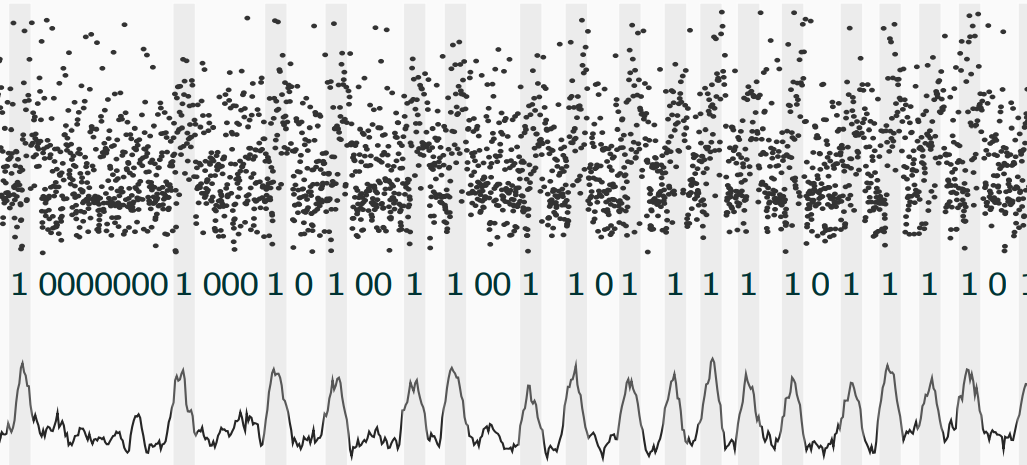
\includegraphics[width=\textwidth]{images/chapter_6/PPSM.PNG}
    \caption{Querying the buffer holding the multiplier $b$. The y axis is a latency scale, and the x axis represent the query index. The dotted plot is a scatter plot while the solid line is the normalized moving average.}
    \label{fig:PPSQ}
\end{figure}

In \Cref{fig:PPSQ} the resulting graph of the querying can be seen, in which the actual bits of the exponent can be clearly detected.

\subsection{Attack Model}
\label{subsec:attackmodel}
We assume that the attacker has no physical access to the device. Moreover, the attacker can only execute unprivileged code on the same machine as victim. Such scenarios in which this happens can be found, for example, when the victim install some malicious program on his machine/smartphone. Another examples can be found in could computing where an attacker has a victual machine on the same physical machine as the victim, or in a web environment in which the attacker runs unprivileged JavaScript code.

In the scope of this chapter we will focus on shared hardware in the form of data/instruction cache. While other shared hardware components can also include the DRAM and the memory bus (memory shared hardware) or the branch prediction unit and the arithmetic logic unit (CPU shared hardware), they are not in the scope of this chapter.

\subsection{Today's CPU Complexity}
\label{subsec:todaycpucomplex}
From 2012 onwards Intel has released a new family of microprocessors every year. Each comes with its own new microarchitectural schemes with new Characteristics. To gain performance upgrade in each new installment, that has on average 5\% increase in performance depending on the feature, very small optimizations, such as caches and branch prediction units are added. Such optimizations are the main reason for a side-channel information leakage to exist. Unfortunately, said optimization often come with no documentation since this is Intel intellectual property. Such lack in documentation makes it harder for an attacker to perform said side-channel attacks.

To emphasize today's CPU complexity, it is said that ``Intel x86 documentation has more pages than the 6502 has transistors"~\cite{IntMan}, with 6502 being a reference to a 8-bit microprocessor, used in Apple II, Commodore 64, Atari 800 and more. It had, in the year 1975, roughly 3510 transistors, while the Intel Software Developer's Manuals is 4844 pages (may. 2018). In a more advance microprocessor, such as the 22-core Intel Xeon Broadwell-E5, more than 7 billion transistors can be found. 

\subsection{Background on Caches}
\label{subsec:backgroundoncaches}
In designing a cache side-channel attack, a proper understanding of how caches work, in great detail, is required. First, we need to acknowledge that the requirements for an 'ideal memory' oppose each other. Such requirements are zero latency, infinite capacity, zero cost and infinite bandwidth. The trade-offs are interconnect: \textbf{Bigger is Slower} - Bigger memory often comes with higher latency, due to the fact the it would take longer to determine the location to retrieve.  \textbf{Faster is Expensive} - A reduction in latency often means that a more expensive technology a needed. For example, SRAM is faster than DRAM, which in turn is faster than Disk memory. However, their cost ratio is the other way around. \textbf{Bandwidth is Expensive} - A wider bandwidth needs to come with additional banks, ports, higher frequency or faster technology. 

In our need to understand the use of caches, we need to examine the different memory technologies and why they are used the way they do. \textbf{DRAM} - Dynamic Random Access Memory is the technology that is often used as the main memory (or RAM), while \textbf{SRAM} - Static Random Access Memory is the technology used in caches. The DRAM latency is higher than the SRAM latency, but is cheaper to make. The main difference in cost arises from the fact that DRAM consist only of one transistor and one capacitor per cell, while the SRAM consist of six transistors per cell. Said difference also mean that DRAM is more dense. Finally, the DRAM cell layout and technology requires to periodically refresh each cell.

Since having Both a large and fast, single level of memory is unlikely, CPU's today are made with multiple levels of storage. The main idea is that progressively bigger and slower storage units are located in higher levels of memory, which are farther from the processor. The motivation for such design is to ensure that most of the data the processor needs is kept in the closer and faster levels.

\begin{figure}
    \centering
    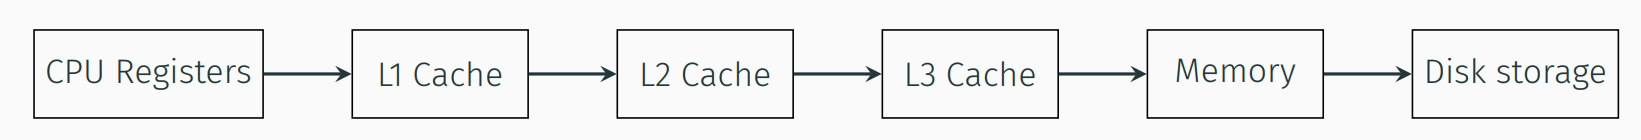
\includegraphics[width=\textwidth]{images/chapter_6/MemHier.PNG}
    \caption{Memory Hierarchy of a common CPU.}
    \label{fig:MemHier}
\end{figure}

The memory hierarchy can be seen in \Cref{fig:MemHier}, where data can reside in, at a given point in time, in the following storage units - in CPU registers, the different levels of the CPU cache, main memory or disk memory. 

\subsection{Caching Basics}
\label{subsec:cachingbasics}
The two main idea of caching is to exploit temporal and spatial locality. \textbf{Temporal Locality} is the notion that a program tends to reference the same memory location many times within a small window of time (for example, loops). The anticipation of such thinking is that recently accessed data will be accessed again soon. Therefor, a good strategy will be to store recently accessed data in automatically managed fast memory. \textbf{Spatial Locality} is the notion that a program tends to reference a cluster of memory locations at a time (for example, sequential instruction access or array traversal). The anticipation will be that surrounding of some accessed data will be accessed soon. A good strategy will consider storing addresses adjacent to the recently accessed one in an automatically managed fast memory. In detail, we want to logically divide memory into equal size blocks (lines) and fetch to cache the accessed block in its entirety.   

Moreover, there are two approaches to the management scheme, manual and automatic. \textbf{Manual Management} means that the programmer manages data movement across levels, which is not scalable for substantial programs. However, it is sometimes used in some embedded systems. \textbf{Automatic management} refer to a scheme in which the hardware itself manages data movement across the different levels in a way that is transparent to the programmer. Meaning that the average programmer does not need to know anything related to the memory hierarchy levels to write a program. On the down side, which begs the question on how to write a fast program if the management is automatic, in addition to what kind of side-channels could arise from such scenario.

The basic unit of storage in the cache is called a block or a line. The main memory is logically divided into cache blocks that map to locations in the cache. And when data is referenced, two outcomes can come of such action - a cache hit or a cache miss. A \textbf{Cache Hit} occurs when a line is referenced and is in the cache. The cached data will be retrieved instead of accessing main memory.  A \textbf{Cache Miss} occurs when a line is referenced and is not in the cache. The data will be fetched from main memory, passing though the cache, possibly eviction other data to ensure enough storage.

When designing a cache, we are faced with a number of design decisions to handle. \textbf{Placement}  - Essentially the place in which we will place or find a block in the cache. \textbf{Replacement} - We need often to remove data from the cache to make room for newer data. Which begs the question of what data to evict. \textbf{Granularity of Management} - The basic units of storage in different levels. Do we store the same amount of blocks across different levels or do we uniformly store the same size of blocks. \textbf{Write Policy} - When a write is being made, we need to decide whether to preform the write operation in all levels or passing the write data to a lower level only upon eviction from that level. \textbf{Instruction/Data} - When a program is executing, the instructions that are in need to be executed are required to be fetched from memory as well. The designer needs to decide whether to treat instruction and data memory as two separate  types or as one of the same.


\subsection{Set-Associative Caches}
\label{subsec:setassoccaches}

We will be focusing on a cache design that is often used in today's CPUs, which is set-associative caches. Which means that the cache will be logically divided into \textbf{Cache Sets}, which will be divided into \textbf{Cache Ways}. Each way will store a cache line worth of data. The division of the memory into different cache sets will be a direct mapping from the memory address. Namely, each address will be associated with a cache set according to a group of bits in the address which will represent the cache set index. The specific way in which the line will is to be fetch will be determine according to the cache replacement policy, since the cache set is expected to be full.  An
abstraction can be seen in \Cref{fig:SetWay}


\begin{figure}
    \centering
    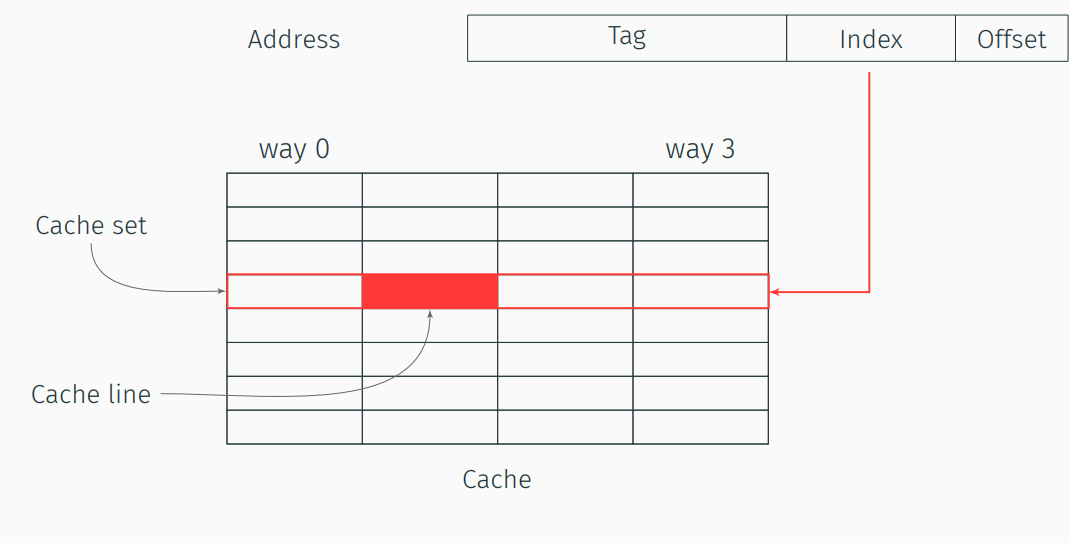
\includegraphics[width=\textwidth]{images/chapter_6/SetWay.PNG}
    \caption{Set-Associative Cache - The set index of a line derives from the set index bits of the address. The cache way is determine according to the cache replacement policy.}
    \label{fig:SetWay}
\end{figure}

Consider the following example: The cache has 8B cache lines, 16 cache sets each consisting of 2 ways. We can compute the set index of the address $(1011111110)_b$ by only looking at bits $b_3, b_4, b_5, b_6$, since we have 16 cache sets (4 bits) and 8 different cache line offset (bits $b_0, b_1, b_2$). Hence the cache set will be $(1111)_b$. We can also compute the size of the whole cache by multiplying the cache dimensions $8 \times 16 \times 2 = 256 $B.

\subsection{Virtual Addresses or Physical Addresses}
\label{subsec:addrorphysicaladdr}
Since we need the bits of address to determine its cache set, we are face with a problem due to the fact that programs running are only aware to the virtual addresses while the hardware side is aware to the physical addresses. The translation between virtual addresses and physical addresses is the responsibility of the MMU (Memory Management Unit).

There are four major ways of implementing such cache mapping according to the addresses. \textbf{VIVT} - Virtually-Indexed, virtually-Tagged. Meaning that there is no need to translate the addresses in order to know the mapping of the addresses into the cache, which is faster. On the other hand, such implementation causes aliasing issues as same virtual address maps to several different physical addresses. This aliasing is due to the tag not being unique, and will force a flush action to the entire cache on context swiching. \textbf{VIPT} - Virtually-Indexed, Physically-Tagged. Meaning that there will be a need for TLB translation for the tag, but can be looked up in parallel. Such mapping can be quiet fast. Moreover, if the set index bits are derived from the page offset, there is no aliasing, but the cache size is limited to the page size multiply by the number of cache sets. VIPT is used in Intel's L1 caches, with the default page size being 4K and each cache line is 64B, resulting in no larger than $2^6 = 64$ sets. \textbf{PIPT} - Physically-Indexed, Physically-Tagged. Meaning that the translation between virtual and physical addresses will have to be preformed, taking up time. On the other hand, no aliasing issues occurs and no required  limitation on the number of sets is present. Typically used in the larger Intel caches - L2 and L3. \textbf{PIVT} - Physically-Indexed, Virtually-Tagged. Meaning that all the limitations of previous ways apply, and is rarely used in practice. 

\subsection{Replacement Policy} 
\label{subsec:replacementpolicy}
We need to decide on a policy according to which a cache line will be evicted in order to make room for incoming data. Many replacement policies exist, namely FIFO (first in, first out), LRU (least recently used), LFU (least frequently used), random, a hybrid and more.

Intel commonly applies a LRU policy or a pseudo-LRU policy (since pure LRU is complex to implement). Which determines that the oldest cache line to be referenced will be evicted, As if each cache line is attached with a time-stamp that is updated on access. An example can be thought of by having $n$ way cache set and $n+1$ different lines of memory that are mapped into said cache set and are accessed in order. The first $1,\dots,n$ lines will fill the cache ways, while the $n+1$ access will evict the first memory line from the set, since all the set ways are full.  

A potential issue arises with LRU policy when a program need to access cyclically $n+1$ memory lines (``program working set") that are mapped to the same $n$ way cache set. This is referenced as a 'set thrasing' and will result in $0\%$ hit rate. If we compare LRU policy to a random policy, depending on the workload, some studies have shown that LRU and random replacement policies have the same hit rate on average.

When implementing a cache side-channel attack, we will normally will want to evict some special memory location from the cache. Considering a non-LRU replacement policy will mean that evicting a memory line from the cache will not necessarily be practical, since there is no guaranty that if the attacker access memory locations in a specific pattern we will evict the whole set from the cache. 
\subsection{Caches on Intel CPUs}
\label{subsec:cachesonintelcpus}
\begin{figure}
    \centering
    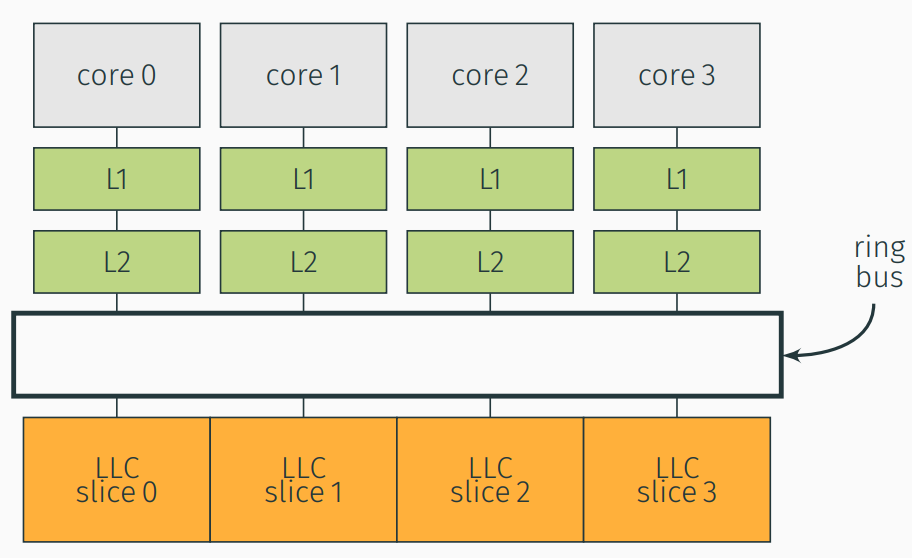
\includegraphics[width=\textwidth]{images/chapter_6/IntelCPU.PNG}
    \caption{Basic Intel CPU - each core has its own L1 and L2 caches, while all connected to a larger sliced L3 cache which can be accessed from all cores. }
    \label{fig:IntelCPU}
\end{figure}

In \Cref{fig:IntelCPU} we can see an abstraction of an Intel CPU architecture, on which every core has its own dedicated L1 instruction and data cache, in addition to a slightly bigger L2. All cores are connected via an interconnected bus to the last level cache (LLC/L3). The LLC often is sliced intro the number of cores, having a dedicated slice to each core, while having all cores being able to access all slices. The common practice is that the different levels of caches are inclusive, meaning that a lower level cache is a super-set of the higher ones.  

In order to preform a cache side-channel attack, an attacker can optimize its cache usage, among other things, using the following command: \texttt{prefetch} - A suggestion to the CPU that some memory line will be accessed soon, can trigger fetching that line into the cache by the CPU. \texttt{clflush} - Cache line flush, instructs the CPU to flush a memory line from all levels of the cache. The two instructions are based on virtual addressed.

The different latencies of the different cache levels, as well as the timing difference between a cache miss and a cache hit, as can be seen in \Cref{fig:cache_hits_misses_hist}, are the main primitives of most cache side-channel attacks that will be discussed by the end of this chapter.  

\section{Cache Attacks Techniques} %ben
\label{sec:cacheattackstech}

Microarchitectural attacks exploit hardware properties that allow inferring information on other processes running on the same system.
In particular, cache attacks exploit the measurable timing difference between the CPU cache and the main memory. They have been the most studied microarchitectural attacks for the past 20 years, and were found to be powerful to derive cryptographic secrets~\cite{Percival2009}. In such attacks, the attacker monitors which memory lines are accessed, not the content of a certain memory line.

\noindent Cache attacks are being used in one of the two following common scenarios:
\begin{itemize}
\item \textbf{Covert channel}: two processes communicating with each other when they are not allowed to do so, e.g., across VMs.
\item \textbf{Side channel attack}: one malicious process spies on benign processes, e.g., steals crypto keys, spies on keystrokes etc. 
\end{itemize}
We will focus on side-channel attacks.

\subsection{Cache Side-Channel Timing Attacks}
\label{subsec:cachesidechanneltiming}
Every timing attack works by the following steps:
\begin{enumerate}
    \item Learn timing of different \textit{corner cases}.
    \item Recognizing these corner cases by timing only.
\end{enumerate}
Here, our corner cases are \textit{hits} and \textit{misses}.

\subsubsection{Building the Histogram}
\label{subsubsec:buildingthehistogram}
The first step towards the attack is to build the histogram of the corner cases, cache hits and cache misses. We measure the time for each case many times in order to get rid of noise. Thus, we have a histogram and we can find a threshold to distinguish the two cases.

\noindent Building the histogram for cache hits is done by the following loop:
\begin{enumerate}
    \item Measure time.
    \item Access variable (always cache hit).
    \item Measure time again.
    \item Update histogram with delta.
\end{enumerate}

\noindent Building the histogram for cache misses is done by the following loop:
\begin{enumerate}
    \item Flush variable (\texttt{clflush} instruction).
    \item Measure time.
    \item Access variable (always cache miss).
    \item Measure time again.
    \item Update histogram with delta.
\end{enumerate}

\noindent Having the two histograms, as in \Cref{fig:cache_hits_misses_hist}, we determine the threshold to be as high as possible such that there will be no cache miss below. 
\begin{figure}[!ht]
    \centering
    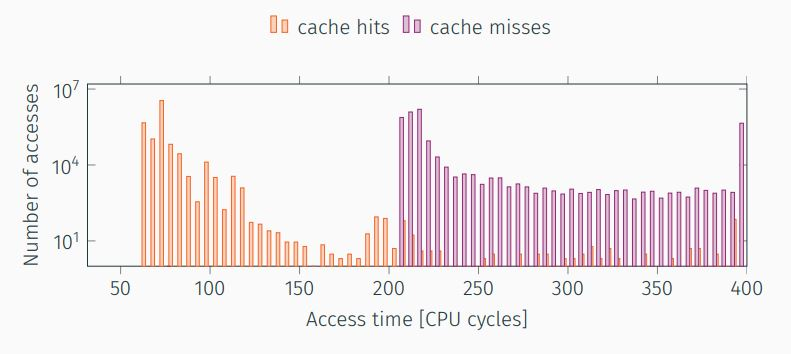
\includegraphics[width=\textwidth]{images/chapter_6/cache_hits_misses_hist.JPG}
    \caption{Timing differences histogram of cache hits and cache misses.}
    \label{fig:cache_hits_misses_hist}
\end{figure}

\subsubsection{How to Measure Time Accurately}
\label{subsubsec:howtomeasuretimeaccuractely}
Consider the fact that the time intervals of our cases is (relatively) very short timings, we ask how to measure time accurately. For such short timings, it is common to use the Time Stamp Counter (TSC) via the unprivileged \texttt{rdtsc} instruction as following:
$$[...] \rightarrow \texttt{rstsc} \rightarrow \mbox{function()} \rightarrow \texttt{rstsc} \rightarrow [...]$$
\noindent By using this instruction, due to out-of-execution, the actual execution order could be different, resulting with wrong measurements. The solution is to use the pseudo-serializing instruction \texttt{rdtscp} or to insert a serializing instruction like \texttt{cpuid} or use to fence instructions like \texttt{mfence}~\cite{benchmark2010}.

We will now introduce two cache attack (main) techniques: Flush+Reload~\cite{Gullasch:2011:CGB:2006077.2006784, Osvik:2006:CAC:2117739.2117741, Yarom2014} and Prime+Probe~\cite{Percival2009,Osvik:2006:CAC:2117739.2117741,Liu:2015:LCS:2867539.2867673}. Both of them are exploitable on x86 and ARM and can be used for both covert channels and side-channel attacks.
\subsection{Flush+Reload}
\label{subsec:flushreload}
The attack is made of four basic steps and it goes as following:
\begin{enumerate}
    \item \textbf{Map. } The attacker maps a shared library (Illustration in \Cref{fig:fr_sharedlib}), by doing that he will have a shared cache line with the victim.
    \item \textbf{Flush.} The attacker \textit{flushes} the shared cache line, it can be done via unprivileged instruction like \texttt{clflush}.
    \item \textbf{Victim.} The attacker lets the victim load (or not load) the shared line, depending on the victim's behaviour.
    \item \textbf{Reload.} The attacker reloads the shared cache line. If the cache line has a \textit{hit} the attacker infers that the victim loaded the data on the previous step, if the cache line has a \textit{miss} the attacker infers that the victim did not load the data on the previous step.
\end{enumerate}

\begin{figure}[!ht]
    \centering
    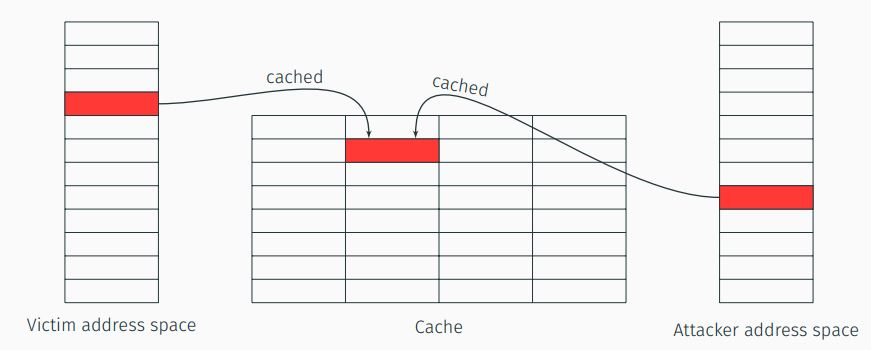
\includegraphics[width=\textwidth]{images/chapter_6/fr_sharedlib.JPG}
    \caption{Attacker maps shared library (shared memory, in cache), shared cache line marked in red}
    \label{fig:fr_sharedlib}
\end{figure}

\begin{figure}[!ht]
    \centering
    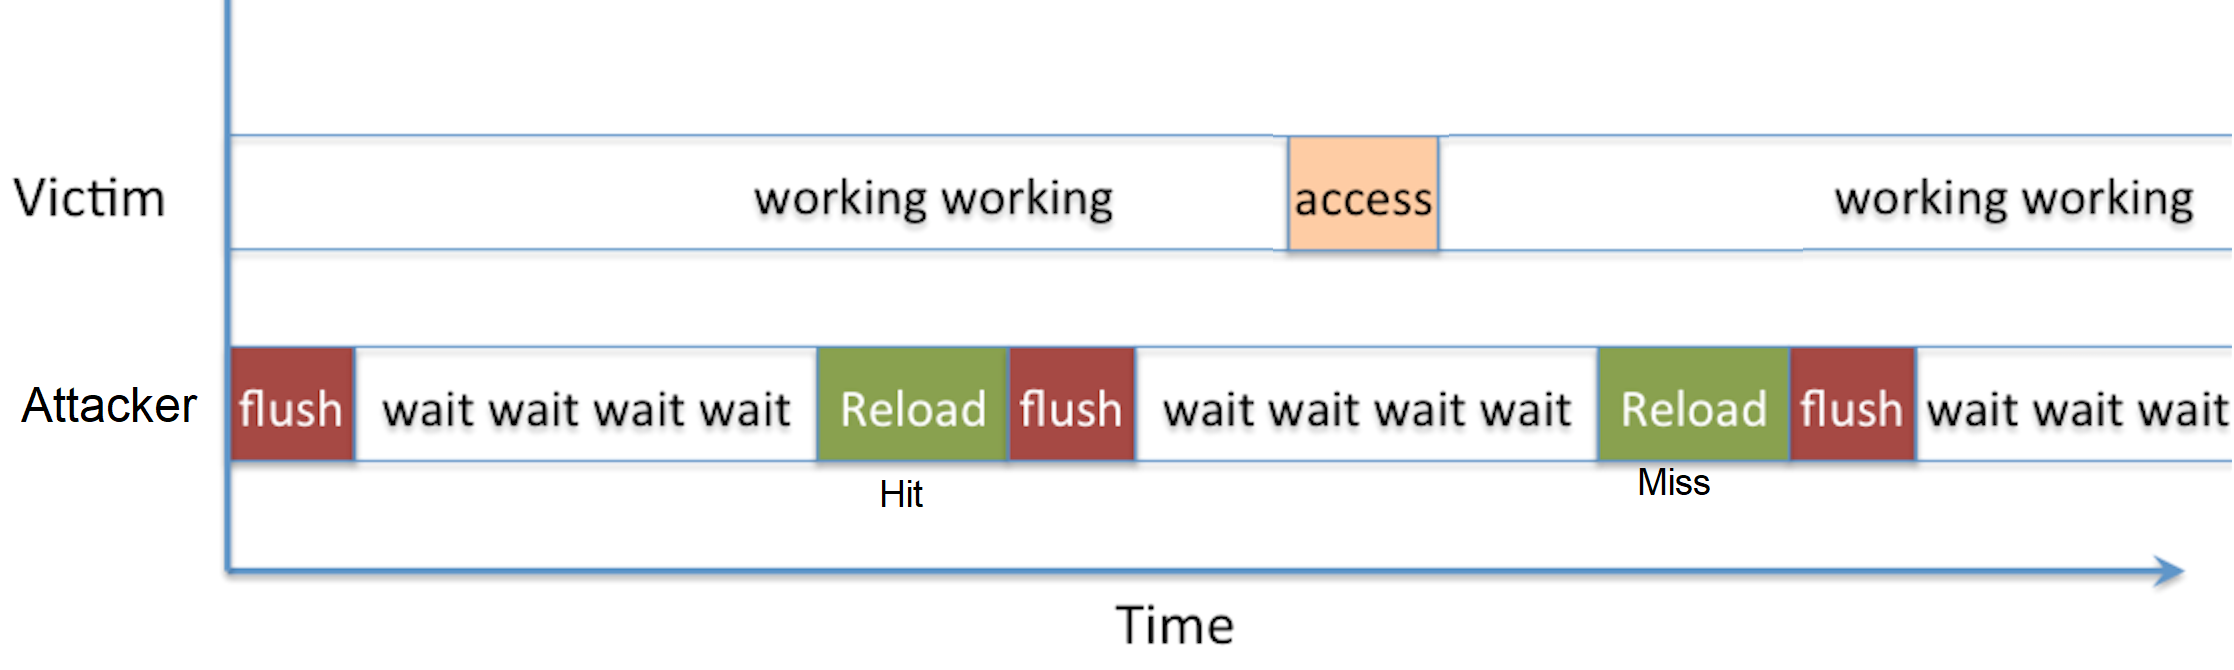
\includegraphics[width=\textwidth]{images/chapter_6/fr_flow.png}
    \caption{Flush+Reload attack flow. Between the first flush and the first reload the victim did not access the shared cache line, so the first reload resulted with a cache hit. Then, after the second flush the victim accessed the shared cache line and hence, the second reload resulted with a miss.}
    \label{fig:fr_flow}
\end{figure}

\noindent The first step (Mapping a shared library) can be done once, while steps 2-4 are repeatable as much as the attacker wants. The main advantage of this attack technique is the fine granularity, which is 1 memory line (usually 64B). On the other hand, this technique is somewhat restrictive, it needs \texttt{clflush} instruction, which is not always available e.g., on ARM-v7 and it needs a shared memory. Illustration of the attack flow in \Cref{fig:fr_flow}.

\subsubsection{Shared Memory}
\label{subsubsec:sharedmemory}
Common method to achieve a shared memory is by a feature called \textit{page-deduplication}. When two different independent processes are loading the same system library, some of their memory pages will be identical, when the operating system (in a cloud scenario - the hypervisor) identify separate identical physical memory pages, if page-deduplication is enabled, it will merge the physical pages in order to save physical memory, and two different virtual memory pages, one of each process, will be mapped into the same physical memory page. As of today, no cloud service company that takes itself seriously is using memory deduplication, e.g., Amazon EC2.

\subsection{Prime+Probe}
\label{subsec:primeprobe}
First, for the Prime+Probe attack to work, the Last-Level-Cache (LLC) should be inclusive, i.e., the LLC is a superset of the L1 cache and the L2 cache. Thus, data evicted from the LLC is also evicted from L1 and L2.
In inclusive caches, a core can evict lines in the private L1 of another core.
The attack is made of the three following steps:
\begin{enumerate}
    \item \textbf{Prime.} The attacker primes the cache by reading memory lines from its own exclusive memory (no shared memory).
    \item \textbf{Victim.} The attacker lets the victim evict (or not evict) lines while running, depending on the victim's behaviour.
    \item \textbf{Probe.} The attacker probes data in a similar way of the prime step but with measurement of how much time it takes to load the lines (Hit / Miss), for each cache set, the attacker determine if the cache set has been accessed.
\end{enumerate}

\begin{figure}[!ht]
    \centering
    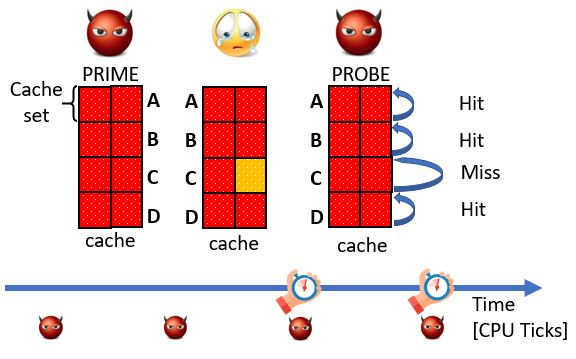
\includegraphics[width=\textwidth]{images/chapter_6/pp_flow.JPG}
    \caption{Prime+Probe flow.}
    \label{fig:pp_flow}
\end{figure}

\noindent In compare to Flush+Reload, this attack technique is less restrictive: it does not require \texttt{clflush}, does not assume shared memory and possible from JavaScript. On the other hand, the granularity is coarser: 1 set.  Illustration of the attack flow in \Cref{fig:pp_flow}.

In practice, we need to evict caches lines without \texttt{clflush} or shared memory, so the following questions arise:
\begin{itemize}
    \item Which addresses do we access to have congruent cache lines?
    \item How do we do that without any privilege?
    \item In which order do we need to access them?
\end{itemize}
For doing that, we need an \textit{eviction set}: addresses in the same set, in the same slice and an \textit{eviction strategy}.

\subsubsection{Eviction Set}
\label{subsubsec:evictionset}
\footnote{From now on, most of the details are correct for a common Intel CPU architecture.}
We want to target the L3 for cross-core attacks and we need addresses that have the same set index. Consider the following cache settings, L3 for a 2-core CPU: 4096 sets, 64B-lines, 12 or 16 ways. Since each memory address indicates one memory byte, the 6 least significant bits of the physical address indicate the line offset. For the sake of simplicity, we assume that the cache is not sliced, since there are $4096=2^{12}$ cache sets, the next 12 bits indicate the cache set. The L3 is physically indexed, so we need to choose addresses with fixed physical address bits. Unfortunately, address translation from virtual to physical is privileged. One of the properties of a virtual address is that a page offset stays the same from virtual to physical address, thus, some of the least significant bits of the virtual address can be used as a sneak peak to the physical address. A typical page size is 4KB, which means just 12 bits of page offset, i.e, 6 bits of line offset and 6 least significant bits of the cache set out of 12. To overcome this limitation, we can use a special type of enlarged pages called \textit{Huge Pages} which are 2MB size each, that is - 21 bits of page offset. This way the set index bits are included in the 21 LSB of the address.

We now have another issue, in practice, the L3 is divided in slices, as many slices as cores. We usually have 2048 sets per slice, that is, actually 11 bits for the set index. We cannot infer the slice number directly from the address, neither from the virtual or the physical. The slice number of each memory line is determined by a hash function which takes all the address bits as input, including physical page number bits (outside the known bits from page offset). Illustration of which bits of the address indicates what for both typical pages and huge pages is shown in \Cref{fig:slicedcache}.

\begin{figure}[!ht]
    \centering
    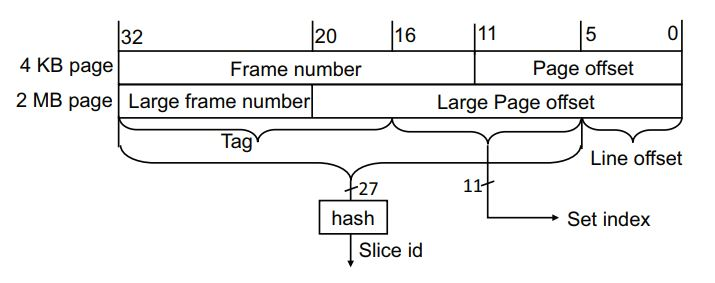
\includegraphics[width=\textwidth]{images/chapter_6/slicedcache.JPG}
    \caption{Sliced cache.}
    \label{fig:slicedcache}
\end{figure}

In addition, the mentioned hash function is undocumented, it designed for performance. But, it does not mean that it is impossible to target the same set in the same slice. Previous work~\cite{EURECOM+4671} showed that the hash function can be reverse engineered, for example in \Cref{fig:hashfunc}.

\begin{figure}[!ht]
    \centering
    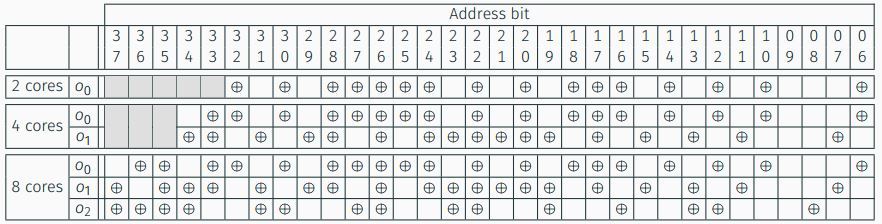
\includegraphics[width=\textwidth]{images/chapter_6/hashfunc.JPG}
    \caption{Three reversed engineered hash functions, depending on the number of cores. Function valid for Sandy Bridge, Ivy Bridge, Haswell, Broadwell}
    \label{fig:hashfunc}
\end{figure}

If the function is unknown, the process will be somewhat slower. But an eviction set can still be achieved via the following algorithm:
\begin{enumerate}
    \item Construct $S$, set of addresses with the same set index.
    \item Access reference address $x \in S$ (to load it in cache).
    \item Iteratively access all elements of $S$.
    \item Measure $t_1$, the time it takes to access $x$. it should be evicted.
    \item Select a random address $s$ from $S$ and remove it.
    \item Iteratively access all elements of $S$\textbackslash$s$.
    \item Measure $t_2$, the time it takes to access $x$ - is it evicted?
    \begin{itemize}
        \item If not, $s$ is part of the same set as $x$, place it back into $S$.
        \item If it was evicted, $s$ is not part of the same set as $x$, discard $s$.
    \end{itemize}
\end{enumerate}
\noindent Note that for a CPU with c cores: $16/c$ addresses in the same set and slice per 2MB page, we can apply the same algorithm with groups of addresses instead of single addresses and speed up the eviction set building process by up to three orders of magnitude.

\subsubsection{Eviction Strategy}
\label{subsubsec:EvictionStrategy}
In the Prime or the Probe step, the attacker evicts a cache set by filling it with $n$ addresses for a $n$-way cache. If the replacement policy is LRU, it access addresses from eviction set 1 by 1. If the replacement policy is not LRU, the eviction rate is lesser than $100\%$, e.g. $75\%$ on Haswell. For non-LRU caches, we can use some heuristics, as in \Cref{fig:haswellstrategy}, that will result with a higher eviction rate.

\begin{figure}[!ht]
    \centering
    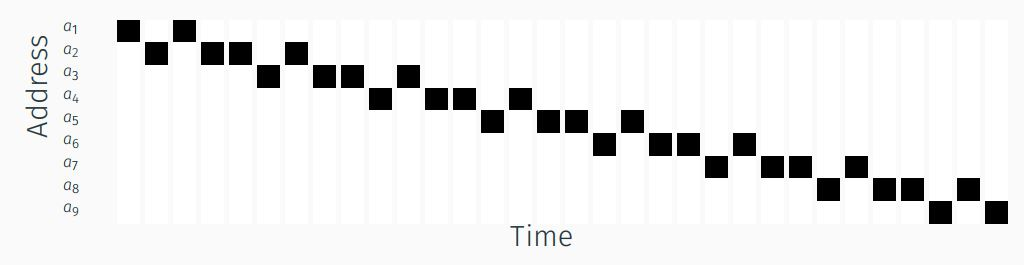
\includegraphics[width=\textwidth]{images/chapter_6/haswellstrategy.JPG}
    \caption{$a_1\dots a_9$ are in the same cache set. Fast and effective on Haswell: eviction rate $> 99.97\%$}
    \label{fig:haswellstrategy}
\end{figure}

\subsubsection{Conclusion}
\label{subsubsec:Conclusion}
To sum it up, in practice, for Prime+Probe on recent processors we need:
\begin{itemize}
    \item An eviction set, i.e., addresses in the same slice and with the same set index. Depends on the addressing.
    \item An eviction strategy, i.e., the order with which we access the eviction set. Depends on the replacement policy
\end{itemize}

\subsection{Hardware vs. implementations}
\label{subsec:Hardwarevsimplementations}

To perform a cache side-channel attack on some software you need two things: First, shared and vulnerable hardware. Note that there will be no side channel if every memory access takes the same time or if you cannot share the hardware component. Second, a vulnerable implementation. Note that a vulnerable implementation doesn't mean that the algorithm is vulnerable. For example, we can take specific implementation of AES and RSA, this doesn't mean that AES and RSA are broken. Not all implementations are created equal.

To sum up, hardware will most likely stay vulnerable, so patch implementations when you can. And remember, constant time is not enough - because an attacker can modify the internal state of the micro-architecture.

\section{Step by Step Attack Demo} %yaniv
\label{sec:stepbystepattack}

The target of the attack in this demonstration, is to get the timestamp of the keystrokes pressed by a user in a gedit program. We only target the timestamps and not the keystrokes themselves, as we are not able to fully recover the pressed keys.

The demonstration is performed on a non-virtualized Linux environment. A requirement to perform the attack is having an Intel CPU, as we need the inclusive property of L3 cache. The code for performing the attack can be cloned from the git repository~\cite{GitClementine}. It is based on the Flush+Reload cache attack that we mentioned in \cref{subsec:flushreload} presented in~\cite{Yarom2014} and~\cite{Gruss2015}.

The attack is performed in 3 steps: calibration, profiling and exploit. For each of these steps, a folder exists in the repository.

\subsection{Step 1: Calibration}
\label{subsec:step1calibration}

In this step we want to create the histogram which depicts the cache misses and hits as a function of the number of CPU cycles. Then we will be able to extract the threshold that will match the CPU on which we perform the attack.
In order to perform the calibration, we run the following commands:

\begin{lstlisting}[language=bash]
  $ cd calibration
  $ make
  $ ./calibration
\end{lstlisting}

The calibration works by generating multiple cache misses and cache hits, and measuring the number of CPU cycles it takes to access a variable. Each of these cases is being performed multiple times in order to get rid of the noise.

\noindent We build a histogram of cache hits and cache misses as described in previous \cref{subsubsec:buildingthehistogram}. The output of the calibration program is a histogram of the cache misses and hits as shown in \Cref{fig:cache_hits_misses_hist}.

We can then find the threshold so it satisfies the following requirements:
\begin{enumerate}
    \item As high as possible
    \item Most cache hits are below it
    \item No cache miss below (we may see one exception due to the way the calibration is coded)
\end{enumerate}

For example, in \Cref{fig:cache_hits_misses_hist}, we can see that there is a clear line in approximately $220$ CPU cycles.

\subsection{Step 2: Profiling}
\label{subsec:step2profiling}

After finding the threshold, we can now profile in order to find the cache lines that are actually useful to get information about the target program. Choosing gedit as the target program, we first need to find the shared library that it uses, so we can give it as an input to the profiler. We then need to find this shared library file location and size. In order to do that, we can use the following one-liner:
\begin{lstlisting}
$ cat /proc/`ps -A | grep gedit | grep -oE "^[0-9]+"`/maps | grep r-x | grep libgedit
\end{lstlisting}
This is equivalent to first finding the pid with
\begin{lstlisting}[language=bash]
  $ ps -A | grep gedit
\end{lstlisting}
and then using this pid in
\begin{lstlisting}[language=bash]
  $ cat /proc/<pid>/maps | grep libgedit
\end{lstlisting}
then copying the line with r-xp permissions (x stands for executable).

Doing that gives the following line (memory range, access rights, offset, –, –, file name):

\begin{lstlisting}[language=bash]
7f2d83197000-7f2d8326d000 r-xp 00000000 08:02 1080575             /usr/lib/gedit/libgedit.so
\end{lstlisting}

Before we can feed the above line to the profiler, we need to update the threshold to the value we found in the calibration step. We can do this by editing the profiler source file (under the profiling directory) and updating the line with the constant 
\begin{lstlisting}[language=bash]
#define MIN_CACHE_MISS_CYCLES
\end{lstlisting}
to the threshold we have.

After updating the threshold, we can run \texttt{make} to compile the profiler. We then use \texttt{sleep 3} so we can have time to trigger the event before the profiler starts, and run the profiler with the line we found above: 
\begin{lstlisting}[language=bash]
sleep 3; ./profiling 200 7f2d83197000-7f2d8326d000 r-xp 00000000 08:02 1080575                    /usr/lib/gedit/libgedit.so
\end{lstlisting}

The profiler does its job by loading the shared library to its address space, and then doing flushes and reloads for each address in the address range given by the offset argument (0 in the above case), and the library size (1080575 bytes) for some given time (200 $\mu$sec for every address in the above command). The output is the number of hits that happened in every address.

The idea is that if a 0 is shown for a given address while triggering the event, then it means that the line in this address was never accessed for this event. Eventually, we will get lines with a number of cache hits, and we want the ones that have at least a non zero value when profiling.

\begin{figure}[!ht]
    \centering
    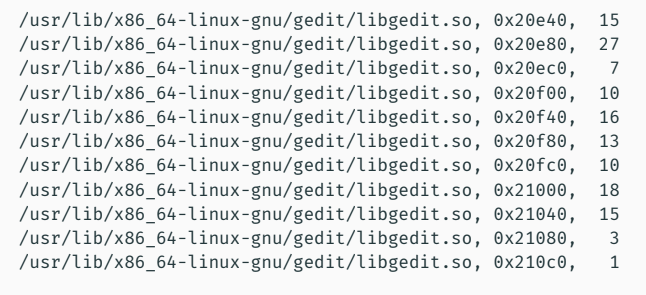
\includegraphics[width=\textwidth]{images/chapter_6/profiling-cache-hits.png}
    \caption{Addresses with cache hits.}
    \label{fig:profiling-cache-hits}
\end{figure}

Running the profiler with offset 0 while jamming a key, doesn't seem to generate cache hits, and we may only see 0. The reason for that, is that the code that handles keystrokes in the library is probably just not in the beginning of the library. Instead (and this is a cheat), we change the starting offset to 20000, and this is approximately where the code that handles keystrokes in the library is found. In real life we will have to wait until we get to something by running the template attack on the whole library. Running the profiler with this new offset, we can see in \Cref{fig:profiling-cache-hits} some addresses that have a non-zero value quite fast. The addresses with the high numbers are the ones we should further investigate in the exploit phase.

\subsection{Step 3: Exploitation}
\label{subsec:step3exploitation}

Equipped with the addresses from the previous step, we can now go to the exploitation dir, change the threshold constant (MIN\_CACHE\_MISS\_CYCLES) as we did for the profiler, and run \texttt{make}. Then we can run the program by 
\begin{lstlisting}[language=bash]
./spy <library-file> <offset>
\end{lstlisting}
giving one of the addresses we found as the offset argument. Starting from the address with the most hits, we can see that even if we are not pressing any key, we are still getting events. The reason for that is that this address is related to the blinking cursor. This is, of course, not really interesting information, and we can understand that it's not always the address that has the most hits that is the most valuable. Trying the next interesting address indeed gives us information about the pressed keys, which is what we wanted to achieve. However, moving the mouse also gives us a lot of hits, which is not perfect. What we will need to do is to inspect the addresses one by one until we find an address that will only work for keystrokes.

We can even further improve the attack by finding the complete matrix of the keystrokes for each of the keys as shown in \Cref{fig:cache-keymap-matrix}. We can see that for different keys, there is a different “signature” of the accessed addresses. Although we may not be able to identify each keystroke precisely, we can try to group the keystrokes to different addresses and eliminate some guesses if we are able to spy on more than one address at a time.

\begin{figure}[!ht]
    \centering
    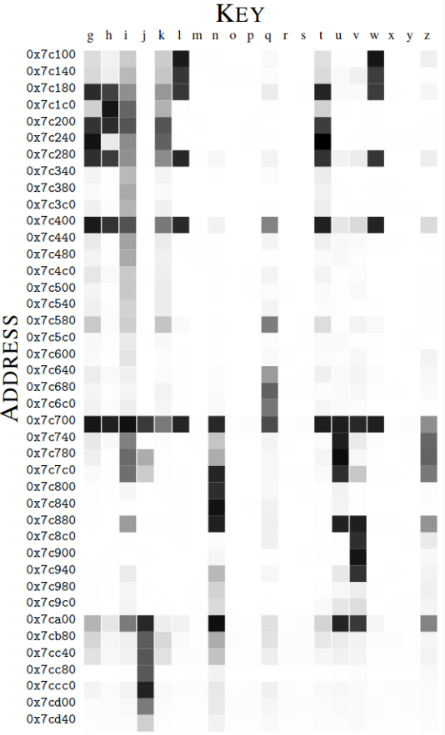
\includegraphics[width=0.8\textwidth]{images/chapter_6/cache-keymap-matrix.png}
    \caption{Complete matrix for each keystroke.}
    \label{fig:cache-keymap-matrix}
\end{figure}

Finally, as it may be annoying to perform the above process manually, we can automate the event triggering and other stuff as shown in~\cite{GitGruss}.